 
% This text is proprietary.
% It's a part of presentation made by myself.
% It may not used commercial.
% The noncommercial use such as private and study is free
% Dec 2007
% Author: Sascha Frank 
% University Freiburg 
% www.informatik.uni-freiburg.de/~frank/
%
% 
\documentclass[handout]{beamer}
%\documentclass[]{beamer}
\setbeamertemplate{navigation symbols}{}
\usepackage{mathtools}  
\usepackage{algorithm}
\usepackage{algpseudocode}

\usepackage{movie15}
\usepackage{amssymb,amsmath}
\usepackage{hyperref}
\usepackage{natbib} 
\usepackage{pgf} 
\usepackage{mathtools}
\usepackage{tikz}
\usepackage{bbm}
%\usepackage{xmpmulti}
% \usepackage{mpmulti}
%\usepackage{appendixnumberbeamer}

% or ...
%\usetheme{Antibes}	% tree outline, neat
%\usetheme{JuanLesPins}	% like Antibes, with shading
%\usetheme{Bergen}	% outline on side
%\usetheme{Luebeck}	% like Warsaw, square sides
%\usetheme{Berkeley}	% interesting left bar outline
\usetheme{Madrid}	% clean, nice.  7/12 page numbers
%\usetheme{Berlin}	% dots show slide number
%\usetheme{Malmoe}	% OK, plain, unshaded
%\usetheme{Boadilla}	% nice, white bg, no top bar
%\usetheme{Marburg}	% nice, outline on right
%\usetheme{boxes}	% ???
%\usetheme{Montpellier}	% tree outline on top, plainish white
%\usetheme{Copenhagen}	% like Warsaw
%\usetheme{PaloAlto}	% looks good
%\usetheme{Darmstadt}	% like Warsaw with circle outline
%\usetheme{Pittsburgh}
%\usetheme{default}
%\usetheme{Rochester}	% like boxy, unshaded warsaw
%\usetheme{Dresden}	% circle outline on top
%\usetheme{Singapore}	% purple gradient top
%\usetheme{Frankfurt}	% like Warsaw with circle outline on top
%\usetheme{Szeged}
%\usetheme{Goettingen}	% light purple right bar outline
%\usetheme{Warsaw}
%\usetheme{Hannover}	% like Goett with bar on left
%\usetheme{compatibility}
%\usetheme{Ilmenau}

%\usecolortheme{lily}

%\newcommand{\bK}{\mathbf{K}}
%\newcommand{\bX}{\mathbf{X}}
%\newcommand{\bY}{\mathbf{Y}}
%\newcommand{\bk}{\mathbf{k}}
%\newcommand{\bx}{\mathbf{x}}
%\newcommand{\by}{\mathbf{y}}
%\newcommand{\bG}{\mathbf{G}}
%\newcommand{\bI}{\mathbf{I}}
%\newcommand{\bg}{\mathbf{g}}
%\newcommand{\bS}{\mathbf{S}}
%\newcommand{\bM}{\mathbf{M}}
%\newcommand{\bw}{\mathbf{w}}
%\newcommand{\eye}{\mathbf{I}}
%\newcommand{\bU}{\mathbf{U}}
%\newcommand{\bV}{\mathbf{V}}
%\newcommand{\bW}{\mathbf{W}}
%\newcommand{\bD}{\mathbf{D}}
%\newcommand{\bZ}{\mathbf{Z}}
%\newcommand{\bu}{\mathbf{u}}
%\newcommand{\bE}{\mathbf{E}}
%\newcommand{\graph}{{\cal H}}

\newcommand{\Perp}{\perp\!\!\! \perp}


\newcommand{\Ep}[2]{\ensuremath{E_{#1}\left[{#2}\right]}}
\def\hpY{\mathbf{\bar{\beta}}}

\newcommand{\gaus}[2]{\mathcal{N}\left({#1};\,{#2}\right)}

\newcommand{\comment}[1]{}

\newcommand{\trace}{\text{trace}}
%\newcommand{\det}{\text{det}}

%\newcommand{\bm}{{\mathbf{m}}}
\newcommand{\loss}{{\cal L}}
\newcommand{\cG}{{\cal G}}
\newcommand{\cV}{{\cal V}}
\newcommand{\cE}{{\cal E}}
\newcommand{\cP}{{\cal P}}
\newcommand{\X}{{\cal X}}
\newcommand{\Y}{{\cal Y}}
\newcommand{\bK}{\mathbf{K}}
\newcommand{\bX}{\mathbf{X}}
\newcommand{\bY}{\mathbf{Y}}
\newcommand{\bk}{\mathbf{k}}
\newcommand{\bx}{\mathbf{x}}
\newcommand{\by}{\mathbf{y}}
\newcommand{\bhy}{\hat{\mathbf{y}}}
\newcommand{\bty}{\tilde{\mathbf{y}}}
\newcommand{\bG}{\mathbf{G}}
\newcommand{\bI}{\mathbf{I}}
\newcommand{\bg}{\mathbf{g}}
\newcommand{\bS}{\mathbf{S}}
\newcommand{\bs}{\mathbf{s}}
\newcommand{\bM}{\mathbf{M}}
\newcommand{\bw}{\mathbf{w}}
\newcommand{\eye}{\mathbf{I}}
\newcommand{\bU}{\mathbf{U}}
\newcommand{\bV}{\mathbf{V}}
\newcommand{\bW}{\mathbf{W}}
\newcommand{\bn}{\mathbf{n}}
\newcommand{\bv}{\mathbf{v}}
\newcommand{\bq}{\mathbf{q}}
\newcommand{\bR}{\mathbf{R}}
\newcommand{\bi}{\mathbf{i}}
\newcommand{\bj}{\mathbf{j}}
\newcommand{\bp}{\mathbf{p}}
\newcommand{\bt}{\mathbf{t}}
\newcommand{\bJ}{\mathbf{J}}
\newcommand{\bu}{\mathbf{u}}
\newcommand{\bB}{\mathbf{B}}
\newcommand{\bD}{\mathbf{D}}
\newcommand{\bz}{\mathbf{z}}
\newcommand{\bP}{\mathbf{P}}
\newcommand{\bC}{\mathbf{C}}
\newcommand{\bA}{\mathbf{A}}
\newcommand{\bZ}{\mathbf{Z}}
\newcommand{\bff}{\mathbf{f}}
\newcommand{\bF}{\mathbf{F}}
\newcommand{\bo}{\mathbf{o}}
\newcommand{\bc}{\mathbf{c}}
\newcommand{\bm}{\mathbf{m}}
\newcommand{\bT}{\mathbf{T}}
\newcommand{\bQ}{\mathbf{Q}}
\newcommand{\bL}{\mathbf{L}}
\newcommand{\bl}{\mathbf{l}}
\newcommand{\ba}{\mathbf{a}}
\newcommand{\bE}{\mathbf{E}}
\newcommand{\bH}{\mathbf{H}}
\newcommand{\bN}{\mathbf{N}}
\newcommand{\bd}{\mathbf{d}}
\newcommand{\br}{\mathbf{r}}
\newcommand{\be}{\mathbf{e}}
\newcommand{\bb}{\mathbf{b}}
\newcommand{\bh}{\mathbf{h}}
\newcommand{\bhh}{\hat{\mathbf{h}}}

\newcommand{\graph}{{\cal H}}
\newcommand{\bayes}{{\cal B}}
\newcommand{\cx}{{\cal X}}
\newcommand{\cg}{{\cal G}}
\newcommand{\cm}{{\cal M}}
\newcommand{\ci}{{\cal I}}
\newcommand{\ct}{{\cal T}}
\newcommand{\co}{{\cal O}}
\newcommand{\ck}{{\cal K}}
\newcommand{\cu}{{\cal U}}
\newcommand{\cv}{{\cal V}}
\newcommand{\ce}{{\cal E}}
\newcommand{\cf}{{\cal F}}
\newcommand{\cb}{{\cal B}}
\newcommand{\cq}{{\cal Q}}
\newcommand{\cd}{{\cal D}}

\newcommand{\btheta}{\boldsymbol{\theta}}
\newcommand{\bpi}{\boldsymbol{\pi}}
\newcommand{\bphi}{\boldsymbol{\phi}}
\newcommand{\bPhi}{\boldsymbol{\Phi}}
\newcommand{\bmu}{\boldsymbol{\mu}}
\newcommand{\bSigma}{\boldsymbol{\Sigma}}
\newcommand{\bGamma}{\boldsymbol{\Gamma}}
\newcommand{\bbeta}{\boldsymbol{\beta}}
\newcommand{\bomega}{\boldsymbol{\omega}}
\newcommand{\blambda}{\boldsymbol{\lambda}}
\newcommand{\bkappa}{\boldsymbol{\kappa}}
\newcommand{\btau}{\boldsymbol{\tau}}
\newcommand{\balpha}{\boldsymbol{\alpha}}
\def\bgamma{\boldsymbol\gamma}

\newcommand{\argmin}{\operatornamewithlimits{argmin}}

%\newcommand{\animal}[2]{\item[\bf #1] {\em #2}}
 \newcommand{\ikron}[1] {\bI\otimes #1}
  \newcommand{\val}{\bar{\bx}}
    \newcommand{\train}[1]{{\phi(\bx_{#1})}}
    \newcommand{\ikronval}[1]{(\ikron{\phi(\val_{#1}))}}
\newcommand{\ikronvalT}[1]{(\ikron{\phi(\val_{#1})^T)}}
\newcommand{\ikrontrainT}{(\ikron{\train{i}^T)}}
\newcommand{\ikrontrain}[1]{(\ikron{\train{#1})}}
\newcommand{\ikrontrainAT}{(\ikron{\phi(\bx)^T)}}
\newcommand{\ikrontrainA}{(\ikron{\phi(\bx))}}
  \newcommand{\half}{\frac{1}{2}}
  \newcommand{\con}{C^{(c)}}
    \newcommand{\ig}{\frac{1}{\gamma}}
      \newcommand{\Bi}{\bB^{-1}}
 \newcommand{\kernel}{\hat{\bK}}    
 \newcommand{\ikrontestT}{(\ikron{\test^T)}}
   \newcommand{\test}{\phi(\bx_*)}

% partial derivatives
 \newcommand{\pardev}[2]{\frac{\partial #1}{\partial #2}}
  \newcommand{\dev}[2]{\frac{d #1}{d #2}}
  \newcommand{\dw}{\delta\bw}
  
    \newcommand{\lab}{\mathcal{L}}
      \newcommand{\unlab}{\mathcal{U}}
      
      
  \newcommand{\ind}{1{\hskip -2.5 pt}\hbox{I}}
  
 \newcommand{\ff}[2]{   \cf_{\prec (#1 \rightarrow #2)}}
 \newcommand{\vv}[2]{   \cv_{\prec (#1 \rightarrow #2)}}
  \newcommand{\dd}[2]{   \delta_{#1 \rightarrow #2}}
    \newcommand{\ld}[2]{   \lambda_{#1 \rightarrow #2}}
    \newcommand{\en}[2]{  \bD(#1|| #2)}
       \newcommand{\ex}[3]{  \bE_{#1 \sim #2}\left[ #3\right]} 
       \newcommand{\exd}[2]{  \bE_{#1 }\left[ #2\right]} 
  
%  \newtheorem{theorem}{Theorem}
%\newtheorem{proposition}{Prop}
%\newtheorem{lemma}{Lemma}
%\newtheorem{lemma-ap}{Lemma}
%\newtheorem{definition}{Definition}
%\newtheorem{corollary}{Corollary}
%\newtheorem{claim}{Claim}
%\newtheorem{claim-ap}{Claim}
%\newcommand{\argmin}[1]{\underset{#1}{\mathrm{argmin}} \:}
\newcommand{\argmax}[1]{\underset{#1}{\mathrm{argmax}} \:}
\DeclareMathOperator*{\Max}{max}
\def\eop {{\noindent\framebox[0.5em]{\rule[0.25ex]{0em}{0.75ex}}}}

\newcommand{\tr}[1]{\ensuremath{\mathrm{tr}\left(#1\right)}}
\def\Xdim{{d}}
\def\Ydim{{D}}
\def\Zdim{{S}}

\setbeamertemplate{itemize subitem}{\tiny\raise1.5pt\hbox{\donotcoloroutermaths$\blacktriangleright$}}
\setbeamertemplate{itemize subsubitem}{\tiny\raise1.5pt\hbox{\donotcoloroutermaths$\blacktriangleright$}}
\setbeamertemplate{enumerate item}{\insertenumlabel.}
\setbeamertemplate{enumerate subitem}{\insertenumlabel.\insertsubenumlabel}
\setbeamertemplate{enumerate subsubitem}{\insertenumlabel.\insertsubenumlabel.\insertsubsubenumlabel}
\setbeamertemplate{enumerate mini template}{\insertenumlabel}

\newcommand{\book}[1]{{\it{#1}}}

\newcommand{\high}[1]{{\color{blue}{#1}}}
\newcommand{\raquel}[1]{{\color{red}{#1}}}



\hypersetup{
	colorlinks=true,
	linkcolor=blue,
	filecolor=magenta,      
	urlcolor=cyan,
	pdftitle={Sharelatex Example},
	bookmarks=true,
	pdfpagemode=FullScreen,
}




\beamersetuncovermixins{\opaqueness<1>{25}}{\opaqueness<2->{15}}
\begin{document}
	\title[CSC411 Lec19]{CSC 411 Lecture 21-22: Reinforcement learning}  
	\author[]{Ethan Fetaya, James Lucas and Emad Andrews}
	\institute[]{University of Toronto}
	%\date{Jan 26, 2016} 
	\date{}
	
	\begin{frame}
	\titlepage
\end{frame}


 \setbeamercovered{invisible}

\section{Introduction}



\begin{frame}\frametitle{Today}\small
\begin{itemize}
\item Learn to play games
\item Reinforcement Learning
\end{itemize}
\vspace{2mm}

% \begin{figure}
% 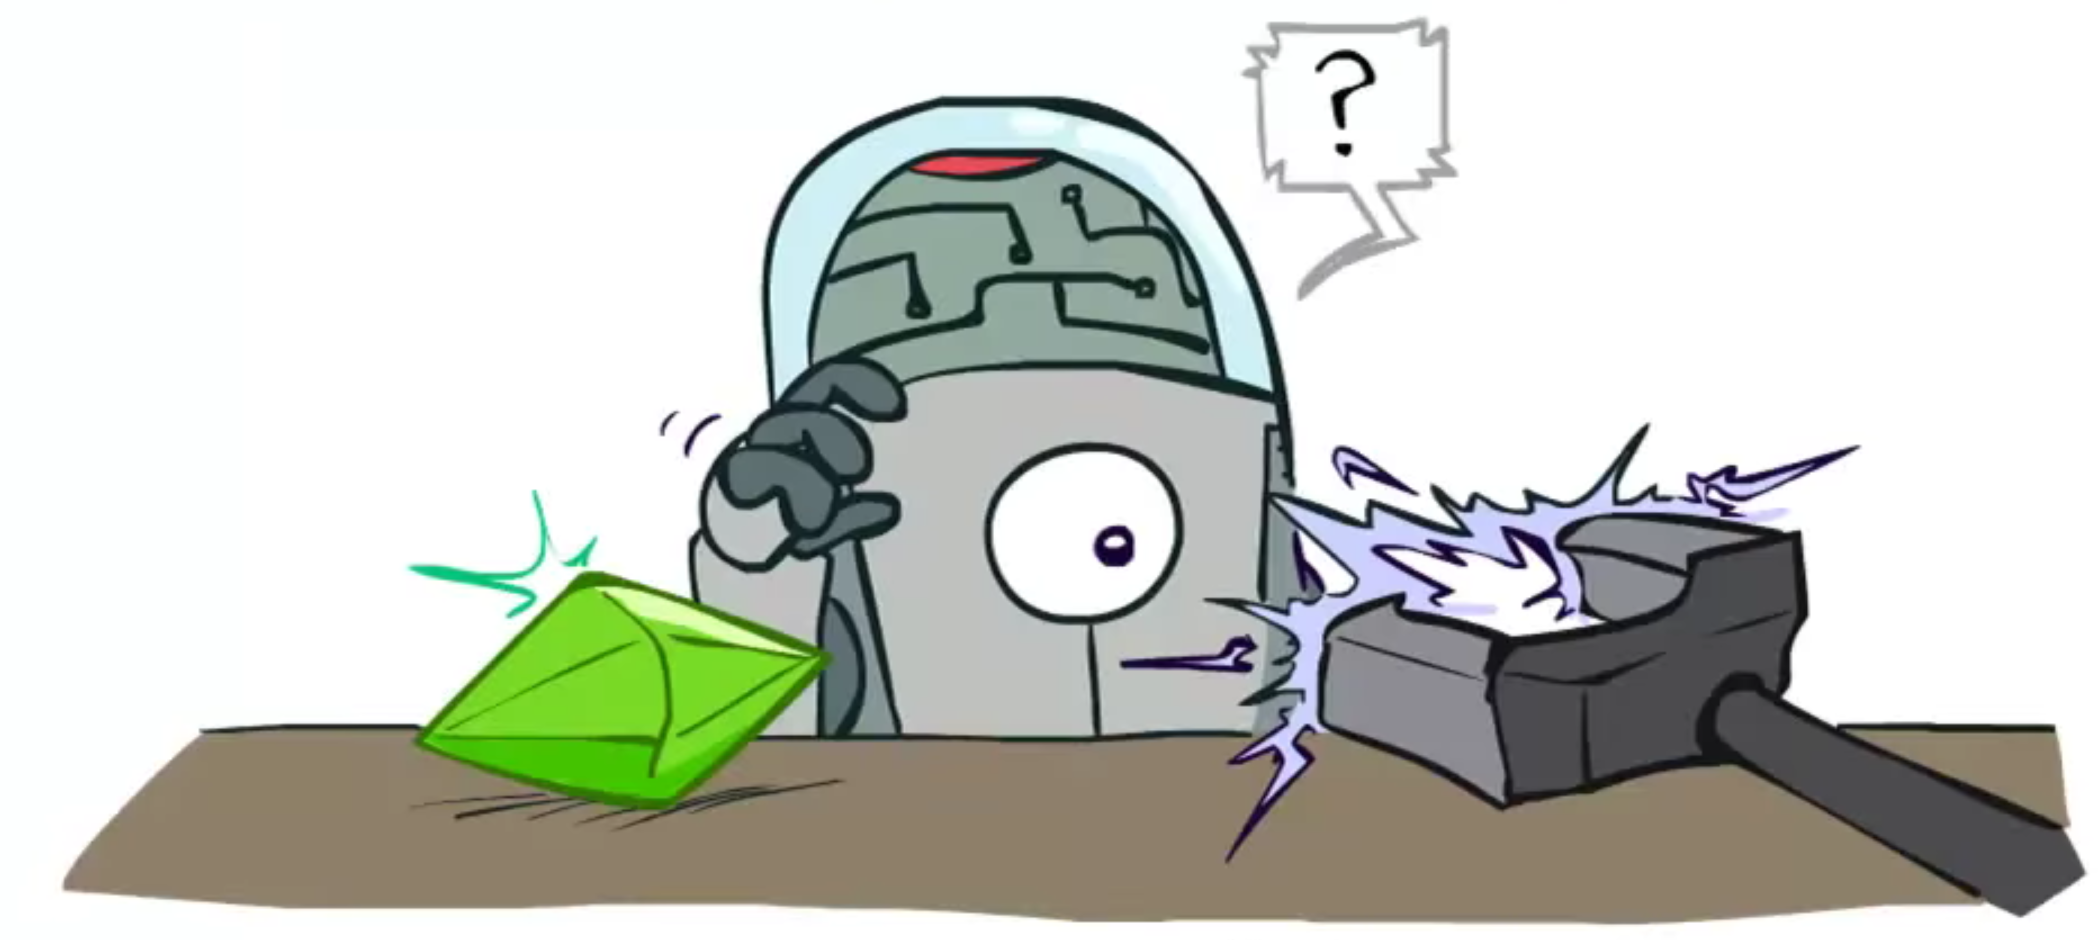
\includegraphics[width =0.78\linewidth]{../old_course_material/slides/figs/lecture19/rll1}
% \end{figure}
% \vspace{2mm}
% 
% \scriptsize [pic from: Peter Abbeel]
\end{frame}

\begin{frame}\frametitle{Playing Games: Atari}\small
\begin{figure}
\href{run:videos/intro/deep_mind.mp4}{
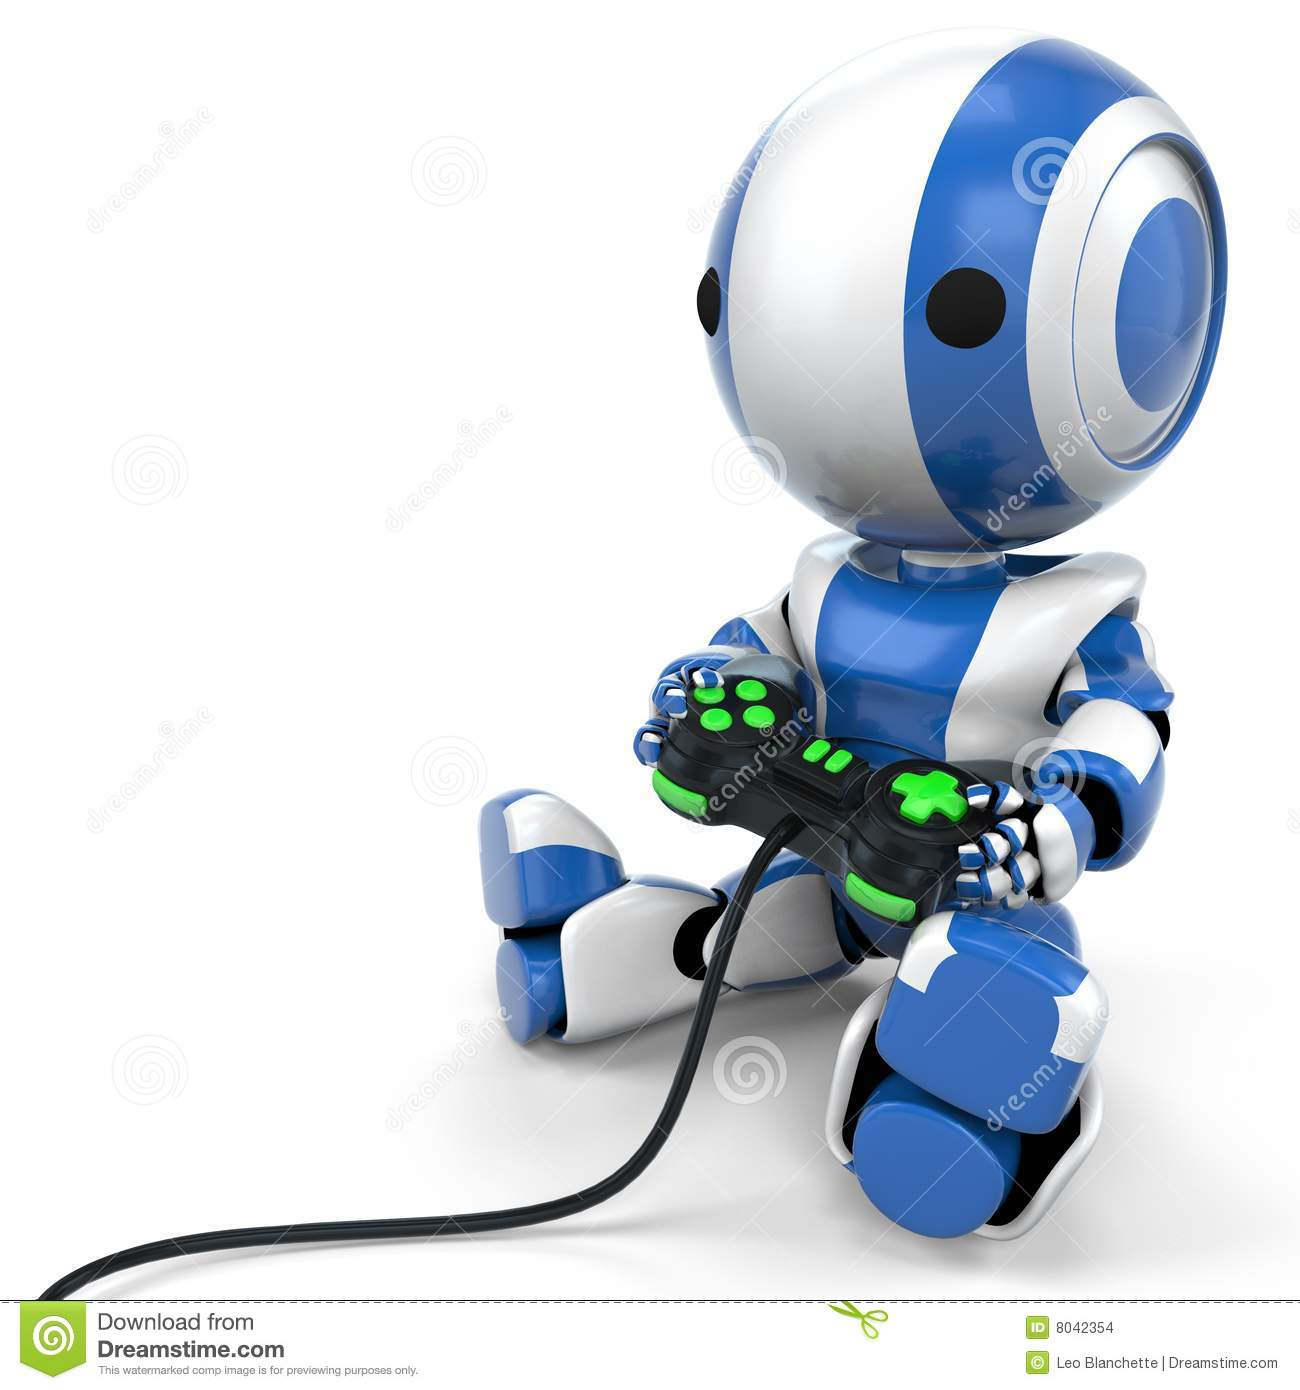
\includegraphics[width =0.6\linewidth,trim=0 69 0 0,clip]{Figures/robot_game.jpg}\\
{\color{magenta}{\url{https://www.youtube.com/watch?v=V1eYniJ0Rnk}}}
}
\end{figure}
\end{frame}

\begin{frame}\frametitle{Playing Games: Super Mario}\small
\begin{figure}
\href{run:videos/intro/super_mario.mp4}{
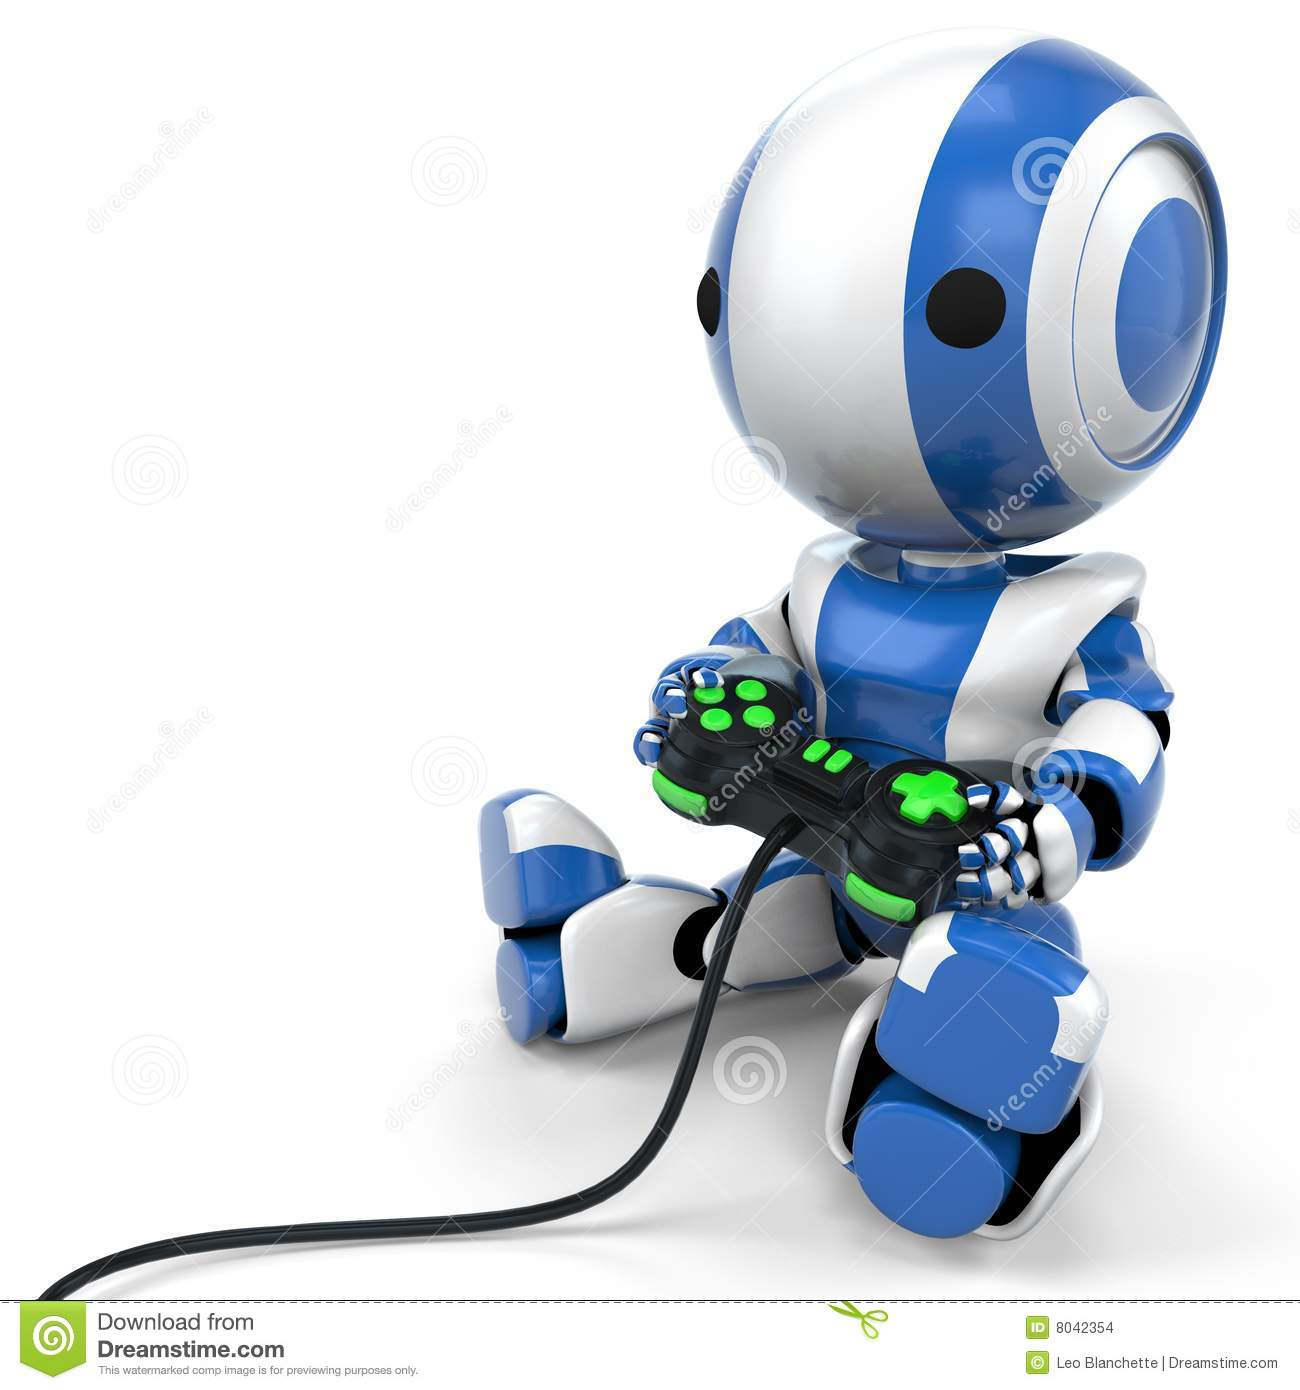
\includegraphics[width =0.6\linewidth,trim=0 69 0 0,clip]{Figures/robot_game.jpg}\\
{\color{magenta}{\url{https://www.youtube.com/watch?v=wfL4L_l4U9A}}}
}
\end{figure}
\end{frame}

\begin{frame}\frametitle{Making Pancakes!}\small
\begin{figure}
\href{run:videos/lecture19/pancakes.mp4}{
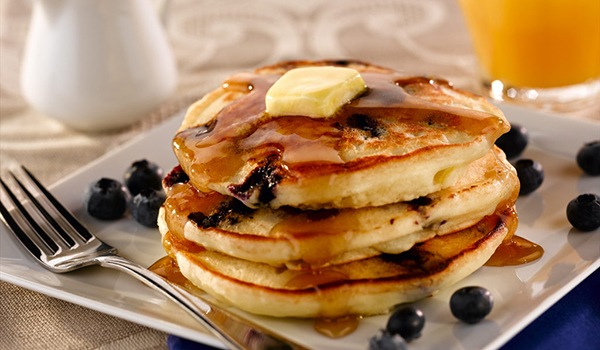
\includegraphics[width=0.9\linewidth]{Figures/pancakes1}\\
{\color{magenta}{\url{https://www.youtube.com/watch?v=W_gxLKSsSIE}}}
}
\end{figure}
\end{frame}


\begin{frame}\frametitle{Reinforcement Learning Resources}\small
\begin{itemize}

\item {\it Reinforcement Learning: An Introduction second edition}, Sutton \& Barto Book (2016)
\item  \href{https://www.youtube.com/watch?v=2pWv7GOvuf0}{Video lectures by David Silver}
\end{itemize}
\end{frame}

% \begin{frame}\frametitle{What is Reinforcement Learning?}\small
% \begin{figure}
% 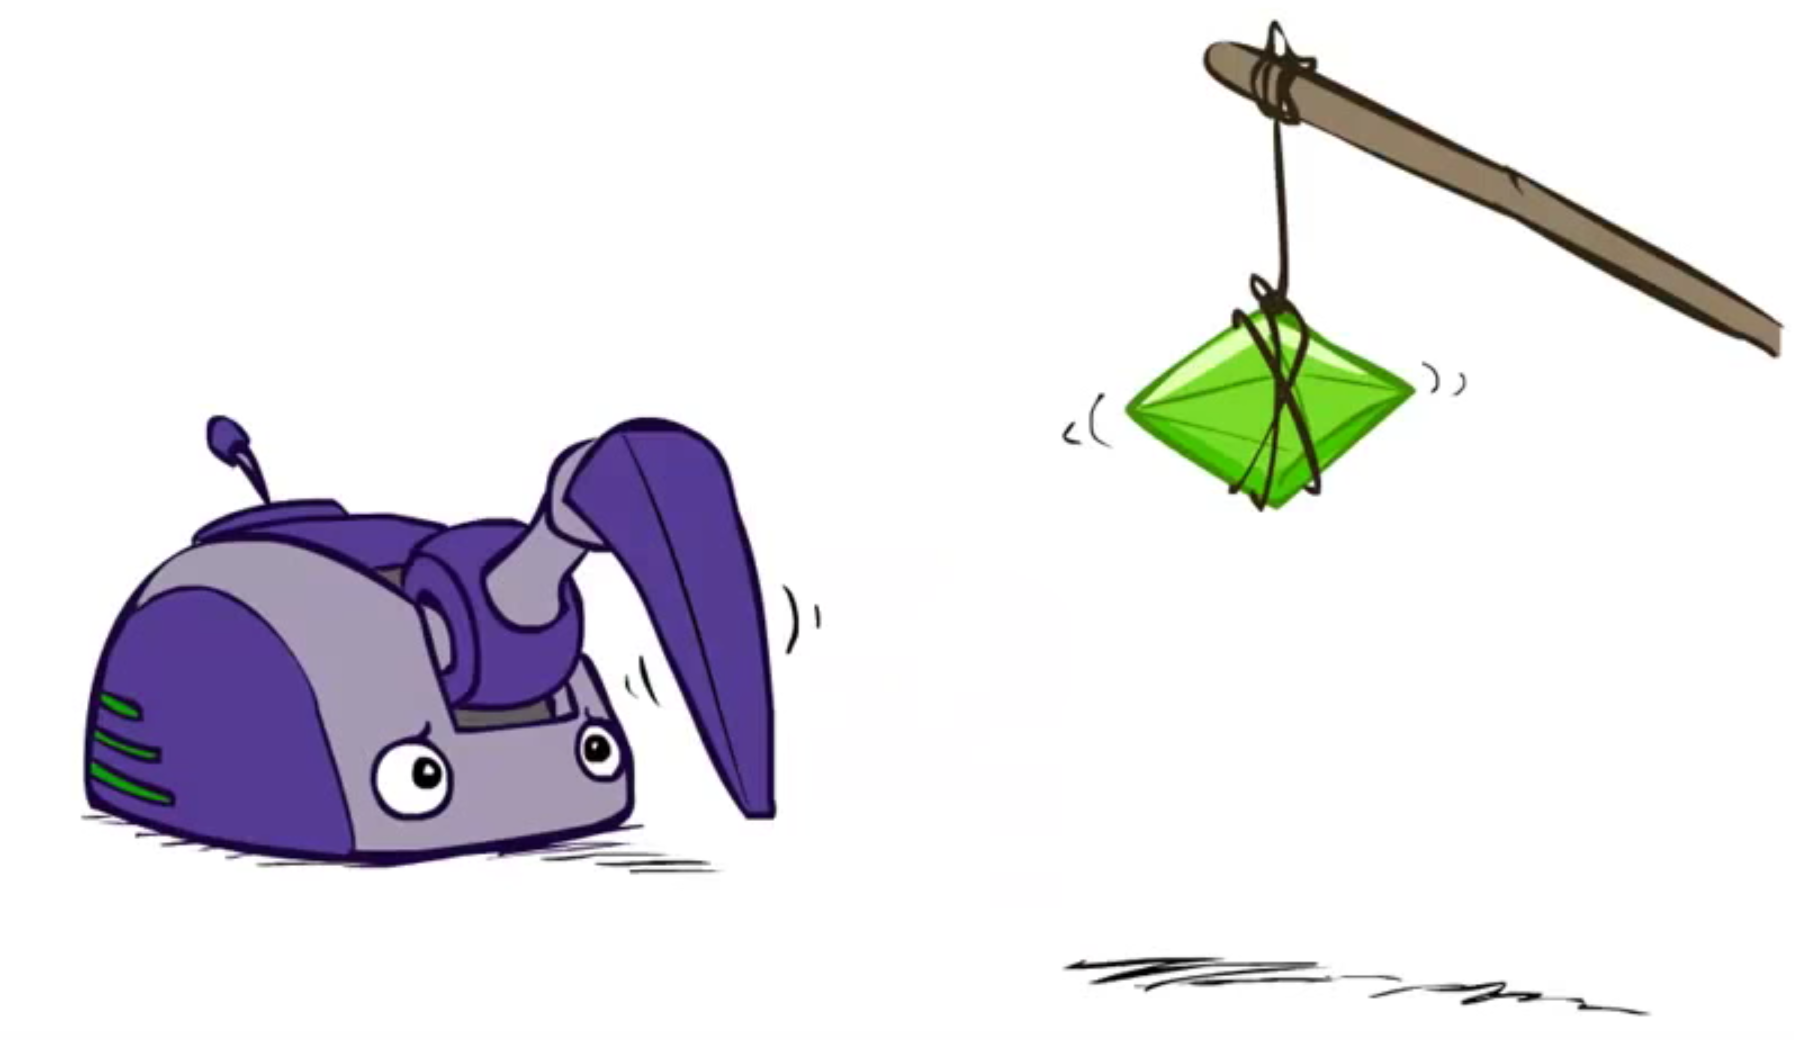
\includegraphics[width=0.9\linewidth]{../old_course_material/slides/figs/lecture19/rll2}
% \end{figure}
% \vspace{5mm}
% \scriptsize [pic from: Peter Abbeel]
% \end{frame}
% 

\begin{frame}\frametitle{Reinforcement Learning}\small
\begin{itemize}
\item Learning algorithms differ in the information available to learner
\begin{itemize}
\onslide<2->\item \high{Supervised}: correct outputs
\onslide<3->\item \high{Unsupervised}: no feedback, must construct measure of good output
\onslide<4->\item \high{Reinforcement learning}: Reward.
\end{itemize}
\onslide<5->\item More realistic learning scenario: 
\begin{itemize}
\item Continuous stream of input information, and actions\\[0.7mm] 
\onslide<6->\item Effects of action depend on state of the world\\[0.7mm] 
\onslide<7->\item Obtain reward that depends on world state and actions\\[0.7mm] 
\begin{itemize}
\onslide<8->\item You know the reward for your action, not other actions.
\onslide<9->\item Could be a delay between action and reward.
\end{itemize}
\end{itemize}
\end{itemize}
\end{frame}

\begin{frame}\frametitle{Reinforcement Learning}\small
\vspace{8mm}

\begin{figure}
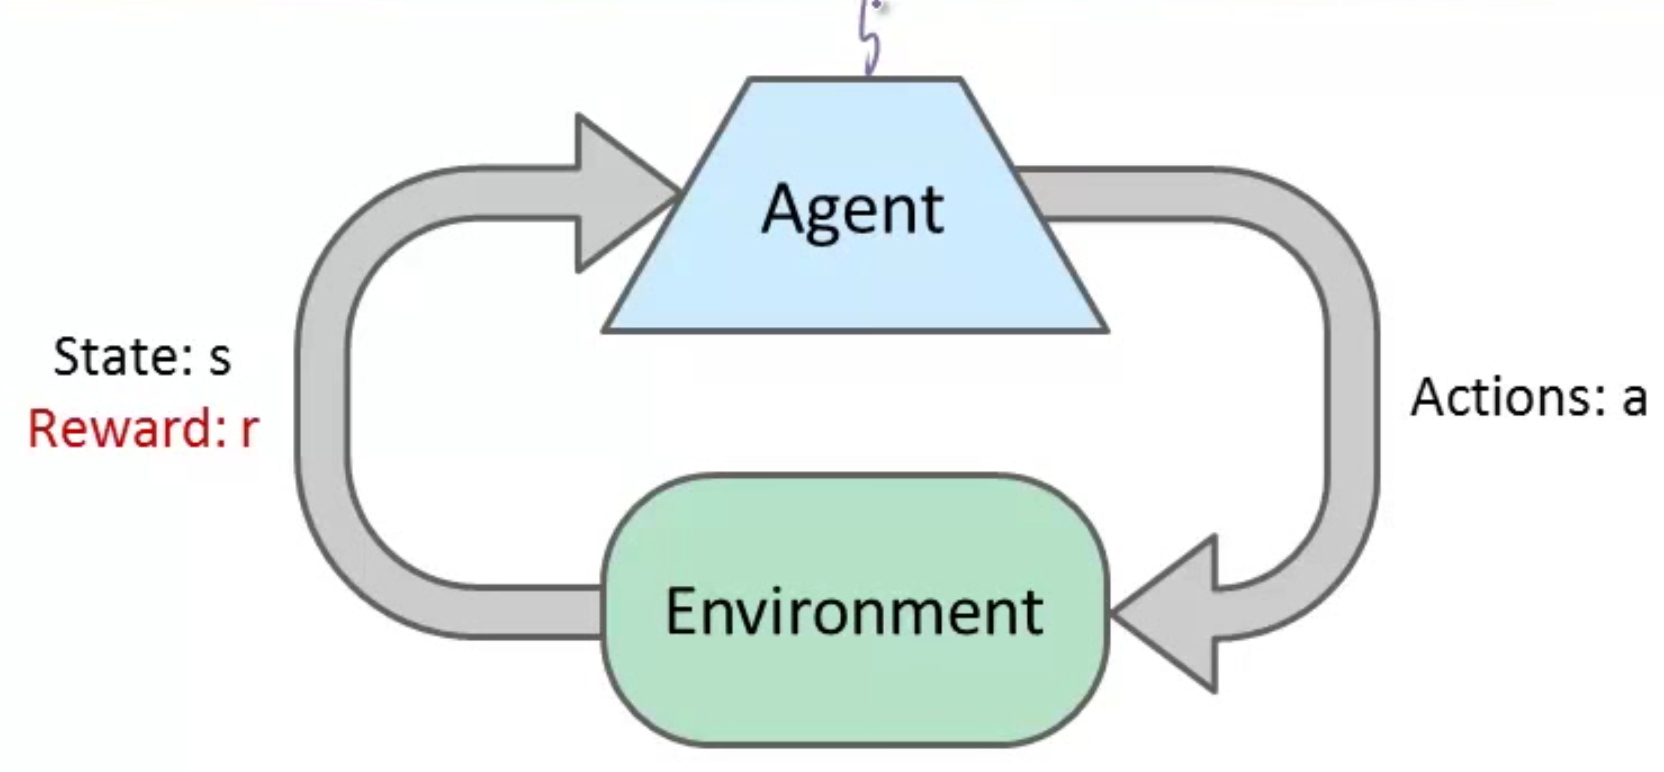
\includegraphics[width=0.85\linewidth]{Figures/rll3}
\end{figure}
\vspace{7mm}

\scriptsize [pic from: Peter Abbeel]
\end{frame}

\begin{frame}\frametitle{Example: Tic Tac Toe, Notation}\small
\vspace{4mm}
\begin{figure}
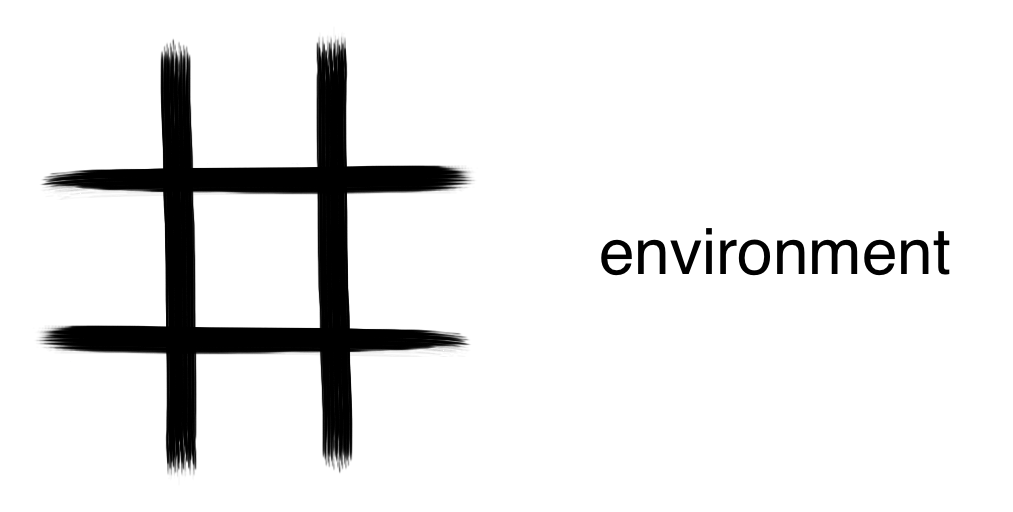
\includegraphics[width=0.75\linewidth]{Figures/tic1d}
\end{figure}
\vspace{5mm}
\end{frame}

\begin{frame}\frametitle{Example: Tic Tac Toe, Notation}\small
\vspace{4mm}

\begin{figure}
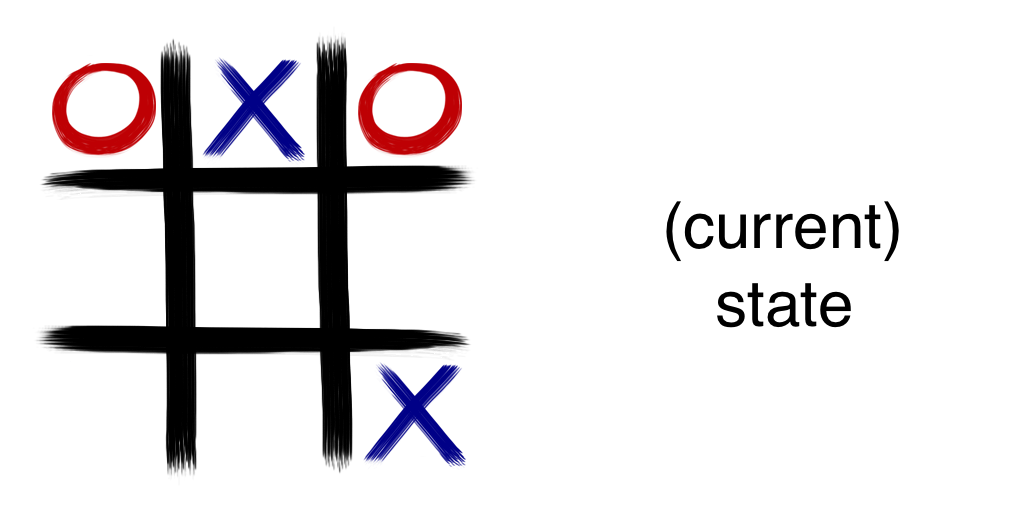
\includegraphics[width=0.75\linewidth]{Figures/tic1c}
\end{figure}
\vspace{5mm}
\end{frame}

\begin{frame}\frametitle{Example: Tic Tac Toe, Notation}\small
\vspace{4mm}

\begin{figure}
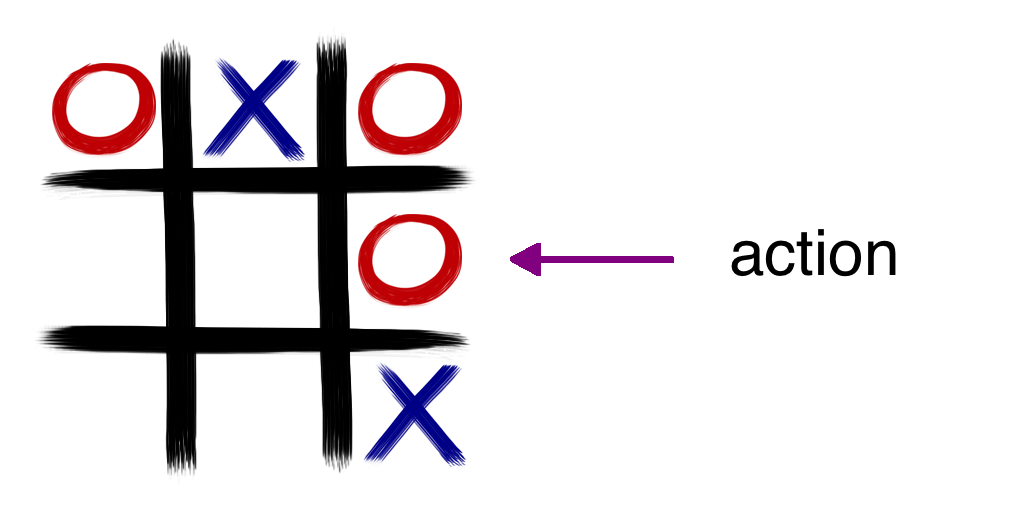
\includegraphics[width=0.75\linewidth]{Figures/tic1b}
\end{figure}
\vspace{5mm}
\end{frame}

\begin{frame}\frametitle{Example: Tic Tac Toe, Notation}\small
\vspace{4mm}

\begin{figure}
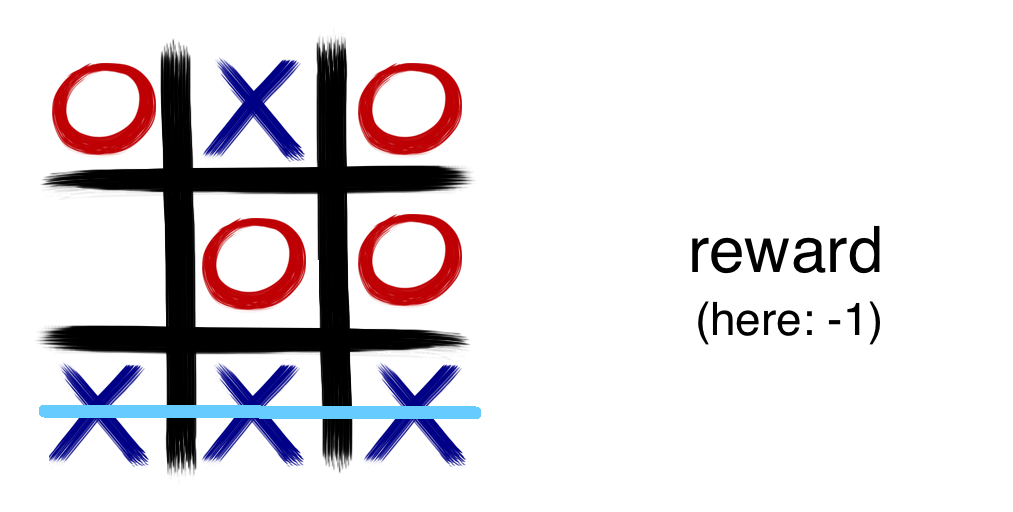
\includegraphics[width=0.75\linewidth]{Figures/tic1e}
\end{figure}
\vspace{5mm}
\end{frame}

\iffalse
\begin{frame}\frametitle{Formulating Reinforcement Learning}\small
\begin{itemize}
\item World described by a discrete, finite set of states and actions
\onslide<2->\item At every time step t, we are in a \high{state} $s_t$, and we:
\begin{itemize}
\onslide<3->\item Take an \high{action} $a_t$ (possibly null action)
\onslide<4->\item Receive some \high{reward} $r_{t+1}$
\onslide<5->\item Move into a new state $s_{t+1}$
\end{itemize}
\onslide<6->\item Decisions can be described by a \high{policy} $\pi$
\begin{itemize}
\onslide<7->\item  a selection of which action to take, based on the current state: $a_t=\pi(s_t)$
\end{itemize}
\onslide<8->\item Aim is to \high{maximize the total reward} we receive over time:
\[
r_{t}+r_{t+1}+r_{t+2}+\dots
\]
\vspace{-4mm}
\onslide<9->\item Sometimes a future reward is discounted by $\gamma^{k-1}$, where $k$ is the number of time-steps in the future when it is received:
\[
r_{t}+\gamma r_{t+1}+\gamma^2 r_{t+2}+\dots
\]
\end{itemize}
\end{frame}
\fi

\begin{frame}\frametitle{Formulating Reinforcement Learning}\small
\begin{itemize}
\item World described by a  set of states and actions
\onslide<2->\item At every time step t, we are in a \high{state} $s_t$, and we:
\begin{itemize}
\onslide<3->\item Take an \high{action} $a_t$ (possibly null action)
\onslide<4->\item Receive some \high{reward} $r_{t+1}$
\onslide<5->\item Move into a new state $s_{t+1}$
\end{itemize}
\onslide<6->\item An RL agent may include one or more of these components:
\begin{itemize}
\item \high{Policy} $\pi$: agent's behaviour function
\onslide<7->\item \high{Value function}: how good is each state and/or action
\onslide<8->\item \high{Model}: agent's representation of the environment
\end{itemize}
\end{itemize}
\end{frame}

\begin{frame}\frametitle{Policy}\small
\begin{itemize}
\item A \high{policy} is the agent's behaviour.
\item It's a selection of which action to take, based on the current state
\item Deterministic policy: $a = \pi(s)$
\item Stochastic policy: $\pi(a|s) = P[a_t = a|s_t = s]$
\end{itemize}

\vspace{30mm}
\scriptsize [Slide credit: D. Silver]
\end{frame}

\begin{frame}\frametitle{Value Function}\small
\begin{itemize}
\item \high{Value function} is the expected future reward
\item Used to evaluate the goodness/badness of states
\onslide<2-> \item Our aim will be to maximize the value function (the total reward we receive over time): find the policy with the highest expected reward
%\item And therefore to select between actions, e.g.
\onslide<3-> \item By following a policy $\pi$, the value function is defined as:
\begin{eqnarray}
V^{\pi}(s_t) &=& \mathbb{E}[r_t + \gamma r_{t+1} + \gamma^2 r_{t+2} + \cdots] \nonumber
\end{eqnarray}
\item $\gamma$ is called a \high{discount rate}, and it is always $0\leq\gamma\leq 1$
\onslide<4->\item If $\gamma$ close to $1$, rewards further in the future count more, and we say that the agent is ``farsighted''
\item $\gamma$ is less than $1$ because there is usually a time limit to the sequence of actions needed to solve a task (we prefer rewards sooner rather than later)
\end{itemize}

\vspace{10mm}
\scriptsize [Slide credit: D. Silver]
\end{frame}


\begin{frame}\frametitle{Model}\small
\begin{itemize}
\item The model describes the \high{environment} by a distribution over rewards and state transitions:
\[
P(s_{t+1}=s', r_{t+1}=r' | s_t = s, a_t = a)
\]
%\item The world and the actor may not be deterministic, or our model of the world may be incomplete
\item We assume the \high{Markov property}: the future depends on the past only through the current state
%\onslide<3->\item We describe the \high{environment} by a distribution over rewards and state transitions:
%\[
%P(s_{t+1}=s', r_{t+1}=r' | s_t = s, a_t = a)
%\]
%\onslide<4->\item The \high{policy} can also be non-deterministic:
%\[
%P(a_t = a | s_t = s)
%\]
%\onslide<5->\item Policy is not a fixed sequence of actions, but instead a conditional plan
\end{itemize}
\begin{figure}
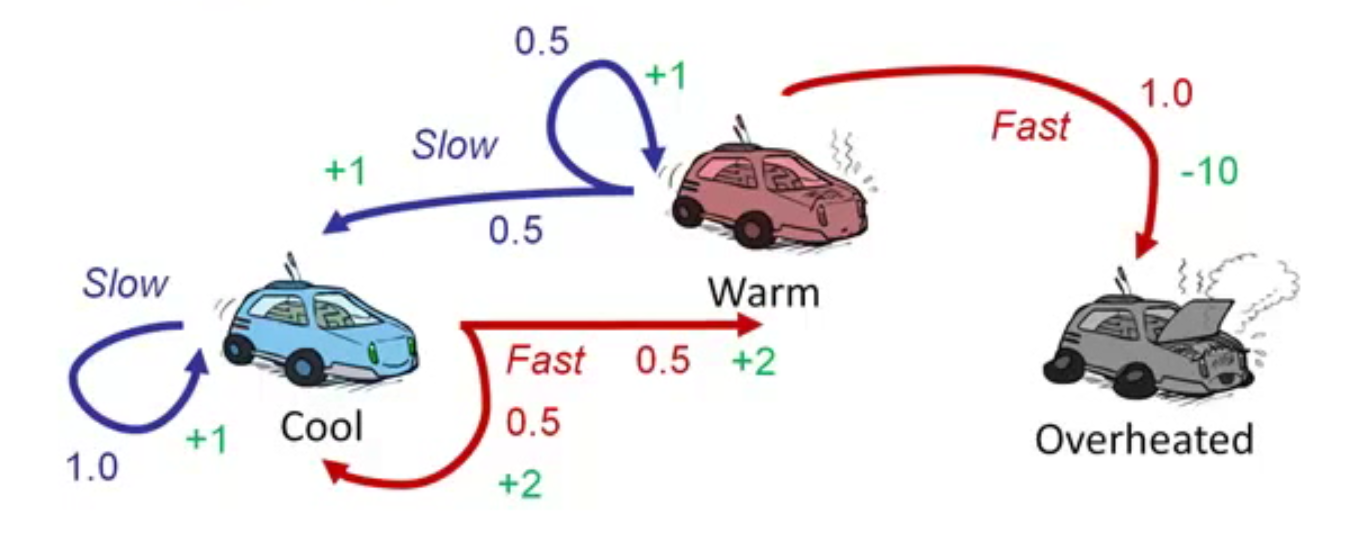
\includegraphics[width=0.7\linewidth]{Figures/rll6} 
\end{figure}
\end{frame}


\begin{frame}\frametitle{Maze Example}\small
\begin{figure}
\begin{minipage}{0.5\linewidth}
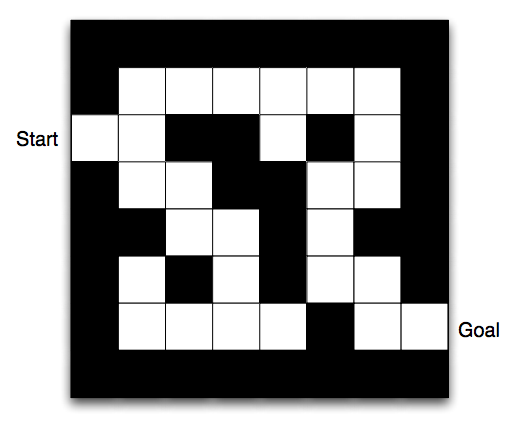
\includegraphics[width=\linewidth]{Figures/maze1}
\end{minipage}
\hspace{3mm}
\begin{minipage}{0.45\linewidth}
\begin{itemize}
\item Rewards: \onslide<2-> $-1$ per time-step
\item Actions: \onslide<3-> N, E, S, W
\item States: \onslide<4-> Agent's location
\end{itemize}
\end{minipage}
\end{figure}

\vspace{12mm}
\scriptsize [Slide credit: D. Silver]
\end{frame}

\begin{frame}\frametitle{Maze Example}\small
\begin{figure}
\begin{minipage}{0.5\linewidth}
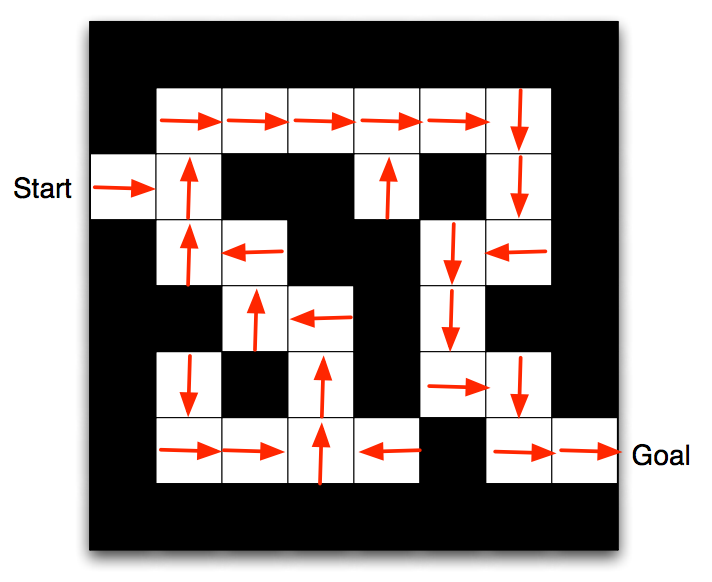
\includegraphics[width=\linewidth]{Figures/maze2}
\end{minipage}
\hspace{3mm}
\begin{minipage}{0.45\linewidth}
\begin{itemize}
\item Arrows represent policy $\pi(s)$ for each state $s$
\end{itemize}
\end{minipage}
\end{figure}

\vspace{14mm}
\scriptsize [Slide credit: D. Silver]
\end{frame}

\begin{frame}\frametitle{Maze Example}\small
\begin{figure}
\begin{minipage}{0.5\linewidth}
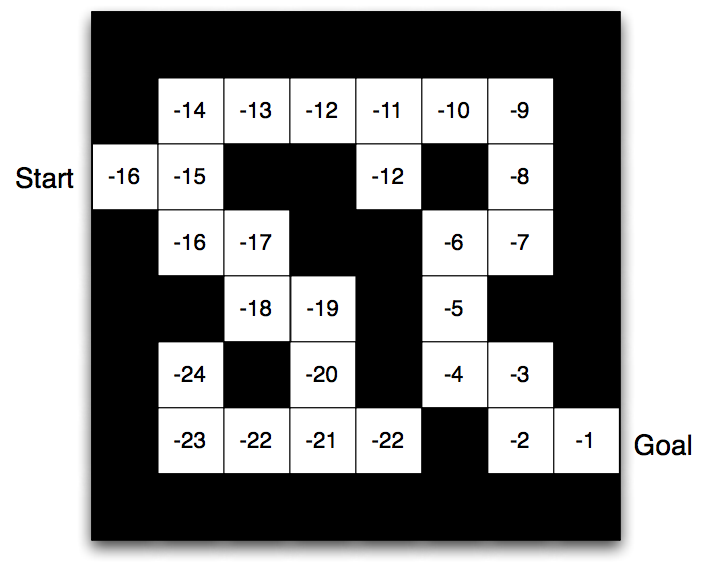
\includegraphics[width=\linewidth]{Figures/maze3}
\end{minipage}
\hspace{3mm}
\begin{minipage}{0.45\linewidth}
\begin{itemize}
\item Numbers represent value $V^{\pi}(s)$ of each state $s$
\end{itemize}
\end{minipage}
\end{figure}

\vspace{14mm}
\scriptsize [Slide credit: D. Silver]
\end{frame}


\iffalse
\begin{frame}\frametitle{Formulating Reinforcement Learning}\small
\begin{itemize}
\item (from previous slide) Sometimes a future reward is discounted by $\gamma^{k-1}$, where $k$ is the number of time-steps in the future when it is received
\item $\gamma$ is called a \high{discount rate}, and it is always $0\leq\gamma\leq 1$
\onslide<2->\item If $\gamma$ close to $1$, rewards further in the future count more, and we say that the agent is ``farsighted''
\onslide<3->\item $\gamma$ is less than $1$ because there is usually a time limit to the sequence of actions needed to solve a task (we prefer rewards sooner rather than later)
\end{itemize}
\end{frame}
\fi

\begin{frame}\frametitle{Example: Tic-Tac-Toe}\small
\begin{itemize}
\item Consider the game tic-tac-toe:
\begin{itemize}
\onslide<2->\item \high{reward}: \onslide<3-> win/lose/tie the game $(+1/-1/0)$ [only at final move in given game]
\onslide<4->\item \high{state}: \onslide<5->positions of X's and O's on the board
\onslide<6->\item \high{policy}: mapping from states to actions 
\begin{itemize}
\onslide<7->\item based on rules of game: choice of one open position
\end{itemize}
\onslide<8->\item \high{value function}: prediction of reward in future, based    on current state
\end{itemize}
\onslide<9->\item In tic-tac-toe, since state space is tractable, can use a table to represent value function 
\end{itemize}
\end{frame}

\begin{frame}\frametitle{RL \& Tic-Tac-Toe}\small
%\vspace{-0.3cm}
\begin{itemize}
\item Each board position (taking into account symmetry) has some probability
\end{itemize}
\begin{minipage}{4cm}
\begin{center}
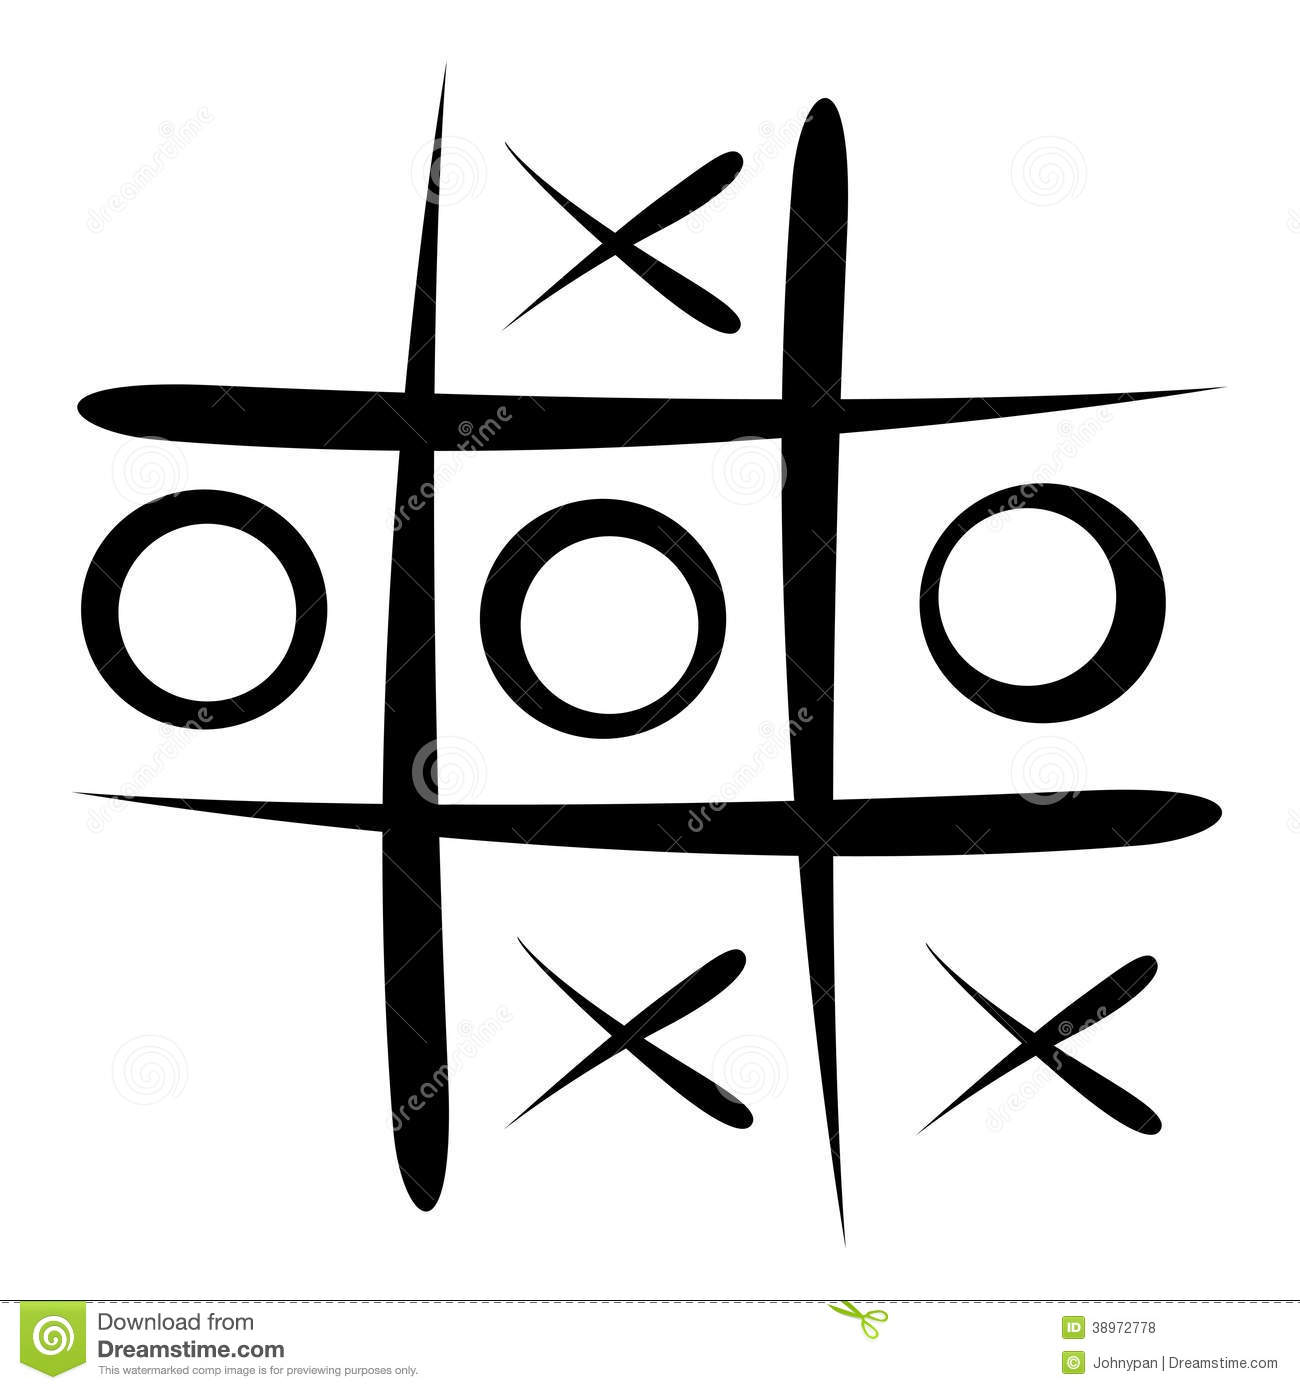
\includegraphics[width=1.0\linewidth]{Figures/tictac} 
\end{center}
\end{minipage}
\begin{minipage}{7cm}
\begin{itemize}
%\item Each board position (taking into account symmetry) has some probability
\onslide<2->\item Simple learning process: 
\begin{itemize}
\onslide<3->\item start with all values = 0.5
\onslide<4->\item \high{policy}: choose move with highest probability of winning given current legal moves from current state
\onslide<5->\item update entries in table based on outcome of each game
\onslide<6->\item After many games value function will represent true probability of winning from each state
\end{itemize}
%\item Can try alternative policy: sometimes select moves randomly (exploration)
\end{itemize}
\end{minipage}
\begin{itemize}
\onslide<7->\item Can try alternative policy: sometimes select moves randomly (exploration)
\end{itemize}
\end{frame}

\iffalse
\begin{frame}\frametitle{Acting Under Uncertainty}\small
\begin{itemize}
\item The world and the actor may not be deterministic, or our model of the world may be incomplete
\onslide<2->\item We assume the \high{Markov property}: the future depends on the past only through the current state
\onslide<3->\item We describe the \high{environment} by a distribution over rewards and state transitions:
\[
P(s_{t+1}=s', r_{t+1}=r' | s_t = s, a_t = a)
\]
\onslide<4->\item The \high{policy} can also be non-deterministic:
\[
P(a_t = a | s_t = s)
\]
\onslide<5->\item Policy is not a fixed sequence of actions, but instead a conditional plan
\end{itemize}
\end{frame}
\fi

\begin{frame}\frametitle{MDP}\small
\begin{itemize}
\item Markov Decision Problem (MDP): tuple $(S,A,P,\gamma)$ where $P$ is
\[
P(s_{t+1}=s', r_{t+1}=r' | s_t = s, a_t = a)
\]
\onslide<2->\item Main assumption: Markovian dynamics and reward.
\onslide<3->\item Standard MDP problems:
\begin{enumerate}
\onslide<4->\item  \high{Planning}: given complete Markov decision problem as input, compute policy with optimal expected return
\begin{figure}
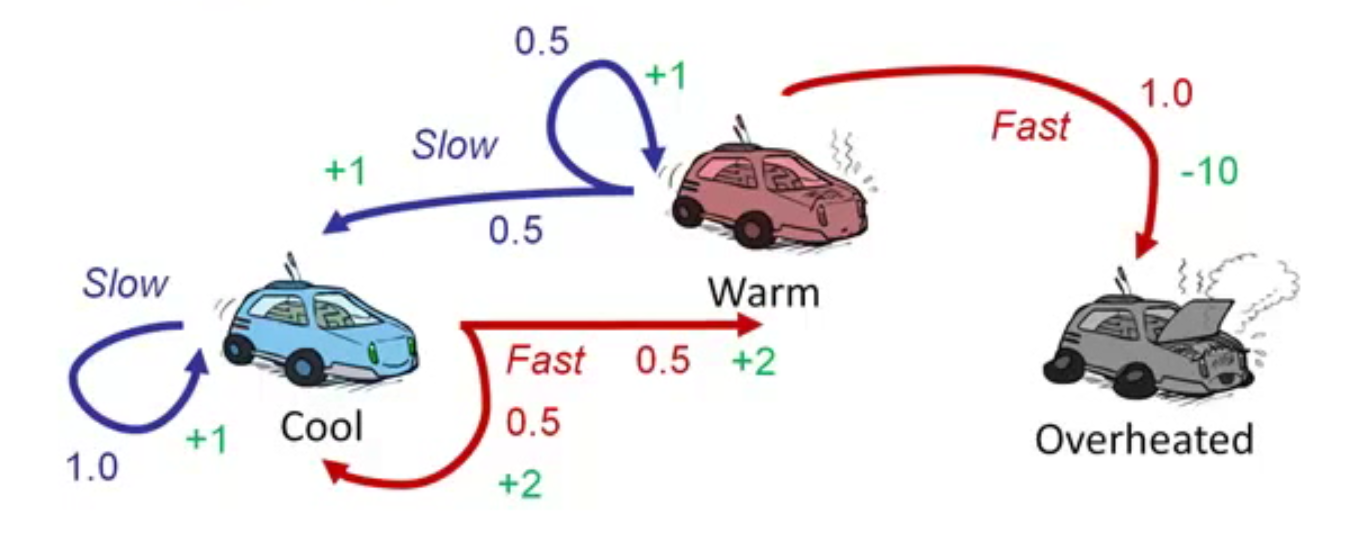
\includegraphics[width=0.7\linewidth]{Figures/rll6} 
\end{figure}
\end{enumerate}
\end{itemize}
\scriptsize [Pic: P. Abbeel]
\end{frame}


\begin{frame}\frametitle{Basic Problems}\small
\begin{itemize}
\item Markov Decision Problem (MDP): tuple $(S,A,P,\gamma)$ where $P$ is
\[
P(s_{t+1}=s', r_{t+1}=r' | s_t = s, a_t = a)
\]
\item Standard MDP problems:
\begin{enumerate}
\item  \high{Planning}: given complete Markov decision problem as input, compute policy with optimal expected return\\[1mm]
\item \high{Learning}: We don't know which states are good or what the actions do. We must try out the actions and states to learn what to do
\end{enumerate}
\end{itemize}
\vspace{28mm}

\scriptsize [P. Abbeel]
\end{frame}

\begin{frame}\frametitle{Example of Standard MDP Problem}\small
\begin{center}
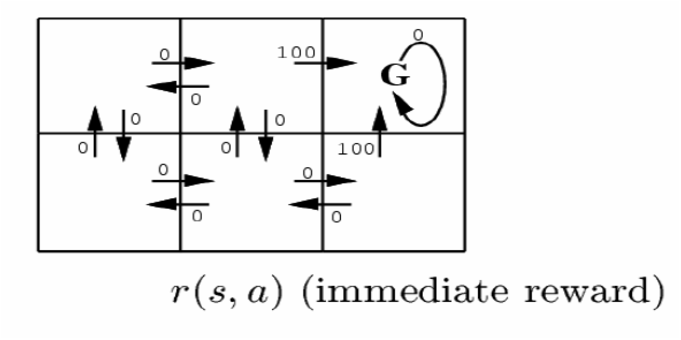
\includegraphics[width=0.54\linewidth]{Figures/tic_tac_rl} 
\end{center}
\begin{enumerate}
\item  \high{Planning}: given complete Markov decision problem as input, compute policy with optimal expected return
\item \high{Learning}: Only have access to experience in the MDP, learn a near-optimal strategy
\end{enumerate}
%We will focus on learning, but discuss planning along the way
\end{frame}

\begin{frame}\frametitle{Example of Standard MDP Problem}\small
\begin{center}
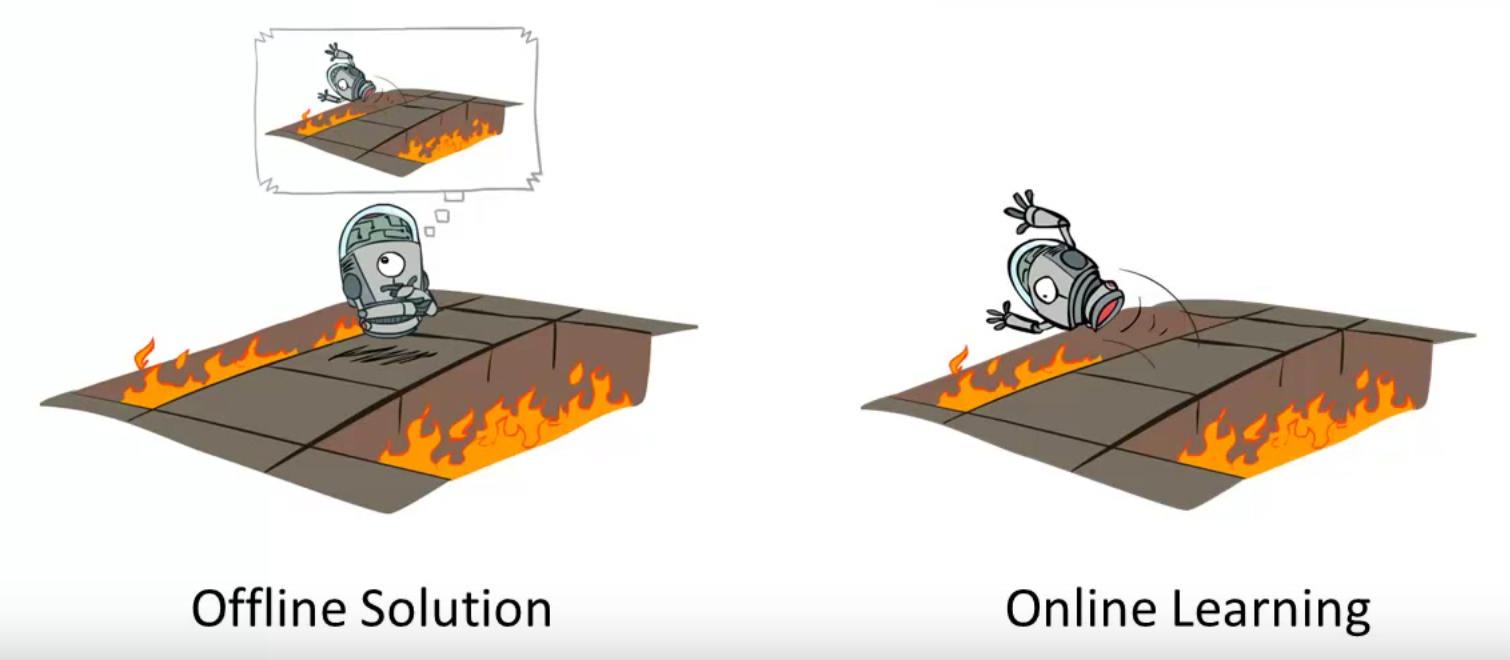
\includegraphics[width=0.785\linewidth,trim=0 50 0 0,clip]{Figures/rll4} 
\end{center}
\begin{enumerate}
\item  \high{Planning}: given complete Markov decision problem as input, compute policy with optimal expected return
\item \high{Learning}: Only have access to experience in the MDP, learn a near-optimal strategy
\end{enumerate}
We will focus on learning, but discuss planning along the way
\end{frame}

\begin{frame}\frametitle{Exploration vs. Exploitation}\small
\begin{itemize}
\item If we knew how the world works (embodied in $P$), then the policy should be deterministic 
\begin{itemize}
\onslide<2->\item  just select optimal action in each state
\end{itemize}
\onslide<3->\item Reinforcement learning is like trial-and-error learning
\onslide<4->\item The agent should discover a good policy from its experiences of the environment
\onslide<4->\item Without losing too much reward along the way

\onslide<5->\item Since we do not have complete knowledge of the world, taking what appears to be the optimal action may prevent us from finding better states/actions
\onslide<6->\item Interesting trade-off: 
\begin{itemize}
\item immediate reward (\high{exploitation}) vs. gaining knowledge that might enable higher future reward (\high{exploration})
\end{itemize}
\end{itemize}
\end{frame}

\begin{frame}\frametitle{Examples}\small
\begin{itemize}
\item Restaurant Selection
\begin{itemize}
\item \high{Exploitation}: Go to your favourite restaurant
\item \high{Exploration}: Try a new restaurant
\end{itemize}
\item Online Banner Advertisements
\begin{itemize}
\item \high{Exploitation}: Show the most successful advert
\item \high{Exploration}: Show a different advert
\end{itemize}
\item Oil Drilling
\begin{itemize}
\item \high{Exploitation}: Drill at the best known location
\item \high{Exploration}: Drill at a new location
\end{itemize}
\item Game Playing
\begin{itemize}
\item \high{Exploitation}: Play the move you believe is best
\item \high{Exploration}: Play an experimental move
\end{itemize}
\end{itemize}
\vspace{1mm}
\scriptsize [Slide credit: D. Silver]
\end{frame}

\begin{frame}\frametitle{Value function}\small
\begin{itemize}
\item The value function $V^\pi(s)$ assigns each state the expected reward 
\[
V^\pi(s)=\underset{a_{t},a_{t+i},s_{t+i}}{\mathbb{E}}\left[\sum_{i=1}^\infty\gamma^{i} r_{t+i} |s_t=s\right]
\]
\onslide<2->\item Usually not informative enough to make decisions.
\onslide<3->\item The $Q$-value $Q^{\pi}(s,a)$ is the expected reward of taking action $a$ in state $s$ and then continuing according to $\pi$.
\[
Q^\pi(s,a)=\underset{a_{t+i},s_{t+i}}{\mathbb{E}}\left[\sum_{i=1}^\infty\gamma^{i} r_{t+i} |s_t=s,a_t=a\right]
\]
\end{itemize}
\end{frame}

\begin{frame}\frametitle{Bellman equations}\small
\begin{itemize}
	\item The foundation of many RL algorithms
	{\footnotesize
	\begin{align*}\footnotesize
	V^\pi(s)&=\underset{a_{t},a_{t+i},s_{t+i}}{\mathbb{E}}\left[\sum_{i=1}^\infty\gamma^{i} r_{t+i} |s_t=s\right] \\
	&=\underset{a_{t}}{\mathbb{E}}\left[r_{t+1} |s_t=s\right]  +\gamma \underset{a_{t},a_{t+i},s_{t+i}}{\mathbb{E}}\left[\sum_{i=1}^\infty\gamma^{i} r_{t+i+1} |s_t=s\right] \\
	& = \underset{a_{t}}{\mathbb{E}}\left[r_{t+1} |s_t=s\right] +\gamma \underset{s_{t+1}}{\mathbb{E}}\left[V^{\pi}(s_{t+1})|s_t=s\right] \\
	& = \sum_{a,r}P^{\pi}(a|s_t)p(r|a,s_t)\cdot r+\gamma \sum_{a,s'}P^{\pi}(a|s_t)p(s'|a,s_t)\cdot V^{\pi}(s')
	\end{align*}}
	\item Similar equation holds for $Q$
		{\footnotesize
		\begin{align*}\footnotesize
		&Q^\pi(s,a)=\underset{a_{t+i},s_{t+i}}{\mathbb{E}}\left[\sum_{i=1}^\infty\gamma^{i} r_{t+i} |s_t=s,a_t=a\right] \\
		& = \sum_{r}p(r|a,s_t)\cdot r+ \gamma\sum_{s'}p(s'|a,s_t)\cdot V^{\pi}(s') \\
		&=\sum_{r}p(r|a,s_t)\cdot r+ \gamma\sum_{a',s'}p(s'|a,s_t)p(a'|s')\cdot Q^{\pi}(s',a')
		\end{align*}}
\end{itemize}
\end{frame}

\begin{frame}\frametitle{Solving Bellman equations}\small
\begin{itemize}
	\item The Bellman equations are a set of linear equations with a unique solution.
	\onslide<2->\item Can solve fast(er) because the linear mapping is a contractive mapping.
	\onslide<3->\item This lets you know the quality of each state/action under your policy - \high{policy evaluation}.
	\onslide<4->\item You can improve by picking $\pi'(s)=\max_a Q^{\pi}(s,a)$ - \high{policy improvement}.
	\onslide<5->\item Can show the iterative policy evaluation and improvement converges to the optimal policy.
	\onslide<6->\item Are we done? \onslide<7-> Why isn't this enough?
	\onslide<8->
	\begin{itemize}
		\item Need to know the model! Usually isn't known.
		\item Number of states is usually huge (how many unique states does a chess game have?) 
	\end{itemize}
\end{itemize}
\end{frame}

\begin{frame}\frametitle{Optimal Bellman equations}\small
\begin{itemize}
	\item First step is understand the Bellman equation for the optimal policy $\pi^*$
	\onslide<2->\item Under this policy $V^*(s)=\max_a Q^*(s,a)$
		{\footnotesize
		\begin{align*}\footnotesize
		V^*(s)& = \max_a\left[\mathbb{E}\left[r_{t+1} |s_t=s,a_t=a\right] +\gamma \underset{s_{t+1}}{\mathbb{E}}\left[V^{*}(s_{t+1})|s_t=s,a_t=a\right]\right] \\
		&= \max_a\left[\sum_{r}p(r|a,s_t)\cdot r+\gamma \sum_{s'}p(s'|a,s_t)\cdot V^*(s')\right] \\
		Q^*(s,a)&=\mathbb{E}\left[r_{t+1} |s_t=s,a_t=a\right]+ \gamma\underset{s_{t+1}}{\mathbb{E}}\left[\max_{a'}Q^{*}(s_{t+1},a')|s_t=s,a_t=a\right] \\
		&= \sum_{r}p(r|a,s_t)\cdot r+\gamma \sum_{s'}p(s'|a,s_t)\cdot\max_{a'} Q^*(s',a')
		\end{align*}}
	\onslide<3-> \item Set on nonlinear equations.
	\onslide<4-> \item Same issues as before.
	
\end{itemize}
\end{frame}


\begin{frame}\frametitle{Q-learning intuition}\small
\begin{itemize}
	\item Q-learning is a simple algorithm to find the optimal policy without knowing the mdoel.
		\onslide<2->\item $Q^*$ is the unique solution to the optimal Bellman equation.
	\[
	Q^*(s,a)=\mathbb{E}\left[r_{t+1} |s_t=s,a_t=a\right]+ \gamma\underset{s_{t+1}}{\mathbb{E}}\left[\max_{a'}Q^{*}(s_{t+1},a')|s_t=s,a_t=a\right]
	\]
	\onslide<3->\item We don't know the model and don't want to update all states simultaneously.
	\onslide<4->\item Solution - given sample $s_t,a_t,r_{t+1},s_{t+1}$ from the environment update your $Q$-values so they are closer to satisfying the bellman equation.
	\begin{itemize}
		\item \high{off-policy} method: Samples don't have to be from the optimal policy.

	\end{itemize} 
	\item Samples need to be diverse enough to see everything - exploration.
\end{itemize}
\end{frame}

\begin{frame}\frametitle{Exploration vs exploitation}\small
\begin{itemize}
	\item Given $Q$-value the best thing we can do (given our limited knowledge) is to take $a=\arg\max_{a'}Q(s,a')$ - \high{exploitation}
	\onslide<2->\item How do we balance exploration with exploitation?
	\onslide<3->\item Simplest solution: $\epsilon$-greedy. 
	\begin{itemize}
		\item With probability $1-\epsilon$ pick $a=\arg\max_{a'}Q(s,a')$ (i.e. greedy)
		\item With probability $\epsilon$ pick any other action uniformly.
	\end{itemize} 
	\onslide<4->\item Another idea - softmax using $Q$ values
	\begin{itemize}
		\item With probability $1-\epsilon$ pick $a=\arg\max_{a'}Q(s,a')$ (i.e. greedy)
		\item With probability $\epsilon$ pick any other action with probability $\propto\exp(\beta Q(s,a))$.
	\end{itemize} 
	\onslide<5->\item Other fancier solutions exist, many leading methods use simple $\epsilon$-greedy sampling.
	
\end{itemize}
\end{frame}


\begin{frame}\frametitle{Q-learning algorithm}\small
\vspace{-0.5cm}
\begin{figure}
	 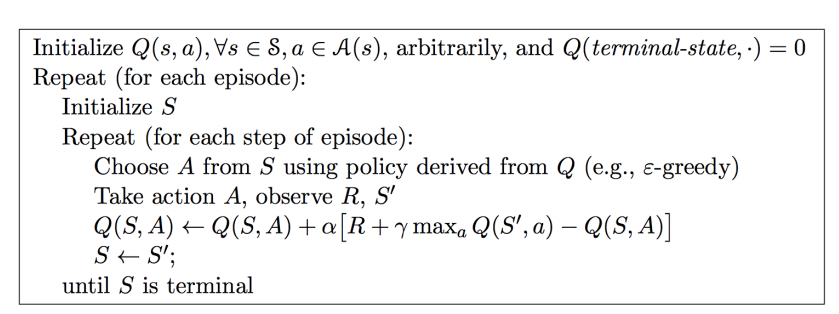
\includegraphics[width=0.9\linewidth]{Qalgo}
 \end{figure}
\vspace{-0.5cm}
\begin{itemize}
	\onslide<2->\item Can prove convergence to the optimal $Q^*$ under mild conditions.
	\onslide<3->\item Update is equivalent to gradient descent on loss $||R+\gamma\max_a Q(S',a)-Q(s,a)||^2$.
	\onslide<4->\item Why $L_2$ loss? Optimal solution is the mean which is what we are looking for!
	
\end{itemize}
\end{frame}

\begin{frame}\frametitle{Bootstrapping}\small

\begin{itemize}
	\item Another way to think about Q-learning.
	\item $Q(s,a)$ is the expected reward, can use Monte-Carlo estimation.
	\onslide<2->\item Problem - you update only after the episode ends, can be very long (or infinite).
	\onslide<3->\item Q-learning solution - take only 1 step forward and estimate the future using our Q value - \high{bootstrapping}.
	\begin{itemize}
		\item "learn a guess from a guess"
	\end{itemize} 
	\onslide<4->\item Q-learning is just one algorithm in a family of algorithms that use this idea.
\end{itemize}
\end{frame}

\begin{frame}\frametitle{Function approximation}\small

\begin{itemize}
	\item Q-learning still scales badly with large state spaces, how many states does a chess game have? Need to save the full table!
	\onslide<2->\item Similar states, e.g. move all chess pieces two steps to the left, at treated as totally different.
	\onslide<3->\item Solution: Instead of $Q$ being a $S\times A$ table it is a parametrized function.
	\onslide<4-> \item Looking for function $\hat{Q}(s,a;\bw)\approx Q^*(s,a)$
	\begin{itemize}
		\onslide<5->\item Linear functions $Q(s,a;\bw)=\bw^T\phi(s,a)$.
		\item Neural network
	\end{itemize}
	\onslide<5->\item Hopefully can generalize to unseen states.
	\onslide<6->\item Problem: Each change to parameters changes all states/actions - can lead to instability.
	\onslide<7->\item For non-linear Q-learning can diverge.
	
\end{itemize}
\end{frame}

\begin{frame}\frametitle{Deep Q-learning}\small

\begin{itemize}
	\item We have a function approximator $Q(s,a;\theta)$, standard is neural net but doesn't have to be.
	\onslide<2->\item What is the objective that we are optimizing?
	\onslide<3->\item  We want to minimize $\mathbb{E}_{\rho}[||R+\gamma\max_{a'} Q(S',a')-Q(s,a)||^2]$
	\begin{itemize}
		\item $\rho$ is a distribution over states, depends on $\theta$!
	\end{itemize}
	\onslide<4->\item Two terms depend on $Q$, don't want to take gradients w.r. to $\gamma\max_aQ(S',a)$
	\onslide<5->\item We want to correct our previous estimation given the new information.
			\vspace{-0.2cm}
	\begin{figure}
		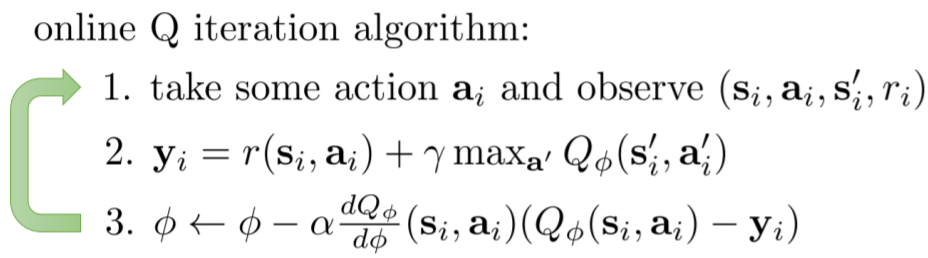
\includegraphics[width=0.85\linewidth]{Qalgo2}
		\vspace{-0.4cm}
		\caption{Take from:rll.berkeley.edu/deeprlcourse}
	\end{figure}
		\vspace{-0.5cm}
	\onslide<5->\item This simple approach doesn't work well as is.
	
	
\end{itemize}
\end{frame}

\begin{frame}\frametitle{Issues and solutions}\small

\begin{itemize}
	\item \high{Problem}: data in the minibatch is highly correlated
	\begin{itemize}
		\item Consecutive samples are from the same eposide and probably similar states.
		\item Solution: \high{Replay memory}.
		\item You store a large memory buffer of previous $(s,a,r,s')$ (notice this is all you need for Q-learning) and sample from it to get diverse minibatch.
	\end{itemize}
	\item \high{Problem}: The data distribution keeps changing
\begin{itemize}
	\item Since we aren't optimizing $y_i$ its like solving a different (but related) least squares each iteration.
	\item We can stabilize by fixing a \high{target network} for a few iterations 
\end{itemize}

\end{itemize}

	\begin{figure}
	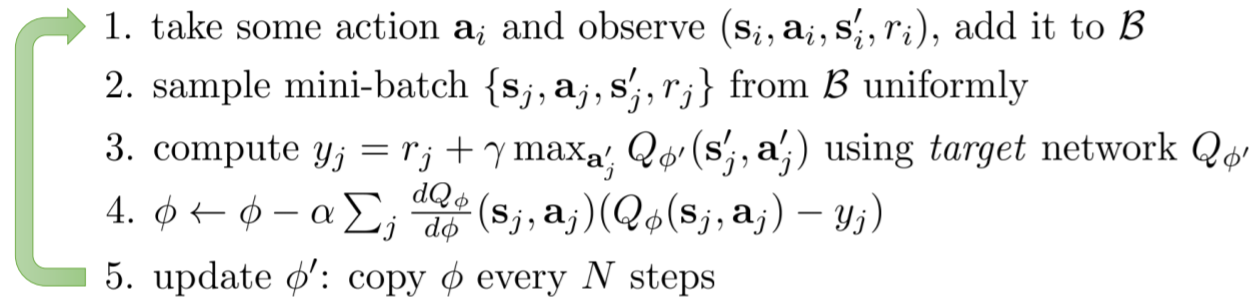
\includegraphics[width=0.75\linewidth]{DQN}
	\vspace{-0.4cm}
	\caption{Take from:rll.berkeley.edu/deeprlcourse}
\end{figure}
\end{frame}

\begin{frame}\frametitle{Example: DQN on atari}\small

\begin{itemize}
	\item Trained a NN from scratch on atari games 

\begin{figure}
	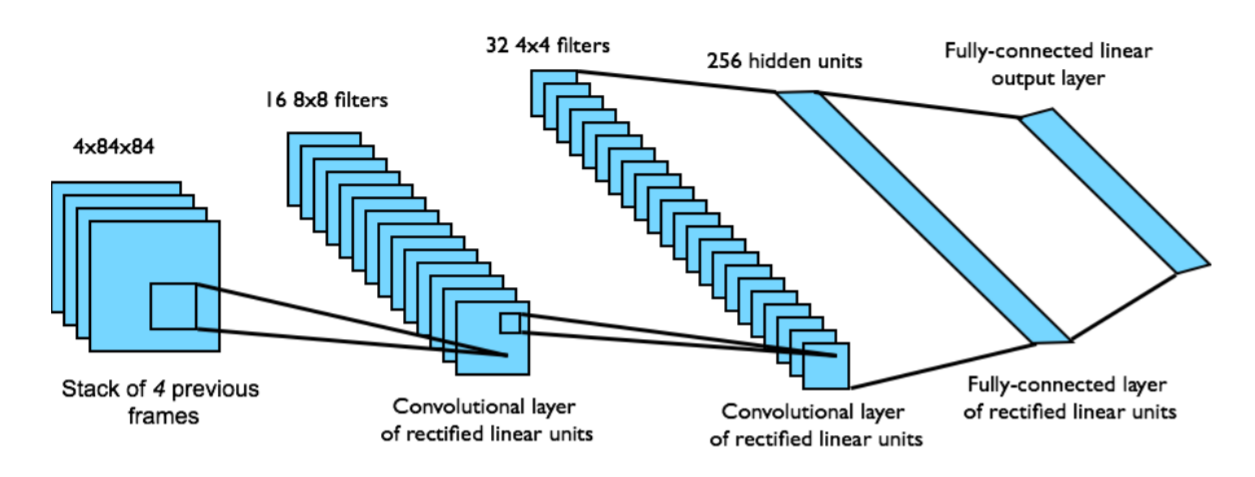
\includegraphics[width=0.75\linewidth]{DQN_arc}
\end{figure}
\onslide<2->\item Ablation study
\begin{figure}
	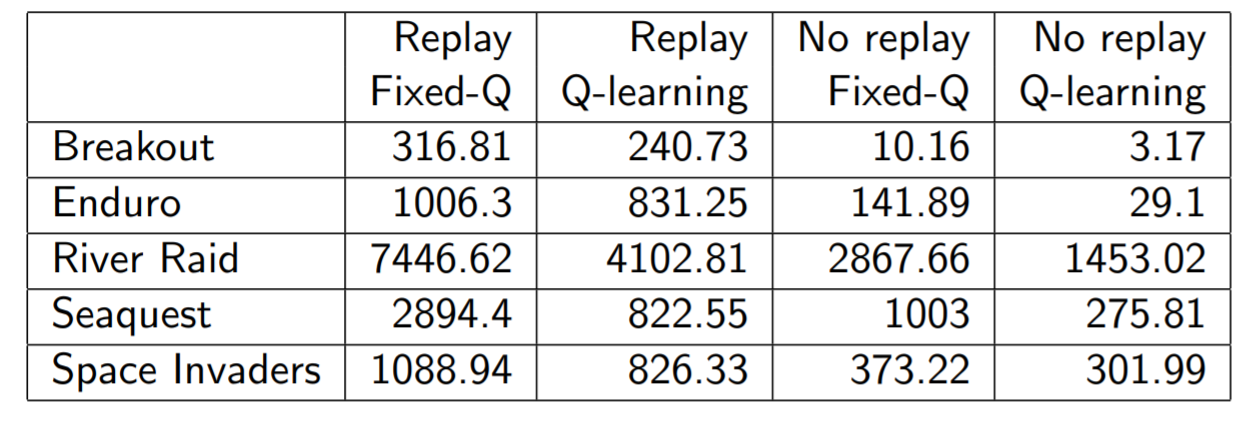
\includegraphics[width=0.75\linewidth]{ablation}
\end{figure}
\end{itemize}

\end{frame}


\begin{frame}\frametitle{RL recap}\small

\begin{itemize}
	\item Learning from experience not from labeled examples.
	\onslide<2->\item Why is RL hard?
	\begin{itemize}
		\onslide<3->\item Limited feedback.
		\onslide<4->\item Delayed rewards.
		\onslide<5->\item Your model effect what you
		 see.
		\onslide<6->\item Huge state space.
	\end{itemize}
	\onslide<7-> \item Usually solved by learning the value function or optimizing the policy (not covered)
	\onslide<8-> \item Model based method but less successful at the moment.
	\onslide<9-> \item How do you define the rewards? Can be trick.
	\begin{itemize}
		\item Bad rewards can lead to \high{reward hacking}
	\end{itemize}
	
\end{itemize}

\end{frame}

\begin{frame}\frametitle{Q-Learning recap}\small

\begin{itemize}
	\item Try to find $Q$ that satisfies the optimal Bellman conditions
	\onslide<2->\item \high{Off-policy} algorithm - Doesn't have to follow a greedy policy to evaluate it.
	\onslide<3->\item \high{Model free} algorithm - Doesn't have any model for instantaneous reward or dynamics.
	\onslide<4->\item Learns a seperate value for each $s,a$ pair - doesn't scale up to huge state spaces.
	\onslide<5->\item Can scale using a function approximation
	\begin{itemize}
		\item No more theoretical guarantees.
		\item Can diverge. 
		\item Some simple tricks help a lot.
	\end{itemize}
	
	
\end{itemize}

\end{frame}


%\begin{frame}\frametitle{}\small
%\begin{itemize}
%\item
%\end{itemize}
%\end{frame}
%
%\begin{frame}\frametitle{}\small
%\begin{itemize}
%\item
%\end{itemize}
%\end{frame}

%
%\begin{frame}\frametitle{Dealing with large datasets}\small
%\begin{itemize}
%\item
%\end{itemize}
%\end{frame}
%
%
%\begin{frame}\frametitle{}\small
%\begin{itemize}
%\item
%\end{itemize}
%\end{frame}
%
%\begin{frame}
%\begin{center}
%\large
%Image features
%\end{center}
%\end{frame}



\end{document}

